
\documentclass{beamer}
\usepackage{cancel}
\usepackage[utf8]{inputenc}
\usepackage{mathtools}
\usepackage{xcolor}
\usepackage{graphicx}
\usepackage[linesnumbered,ruled,vlined]{algorithm2e}
\newcommand\mycommfont[1]{\footnotesize\ttfamily\textcolor{blue}{#1}}
\SetCommentSty{mycommfont}

\setcounter{tocdepth}{2}

\usetheme{Warsaw}
\useoutertheme{infolines}
\usepackage{tikz}
\newcommand\RBox[1]{%
  \tikz\node[draw,rounded corners,align=center,] {#1};%
}  
\author[Elm S. \& Karthe T. \& Golebiewski D. \& Schröder M.E.]
{%
   \texorpdfstring{
        \begin{columns}
            \column{.45\linewidth}
            \centering
            \RBox{Elm S.\\
            \href{mailto:sebastian.elm@tuhh.de}{sebastian.elm@tuhh.de}}
            \column{.45\linewidth}
            \centering
            \RBox{Karthe T.\\
            \href{mailto:thobias.karthe@tuhh.de}{thobias.karthe@tuhh.de}}
        \end{columns}
        \vspace{0.5cm}
        \begin{columns}
            \column{.45\linewidth}
            \centering
            \RBox{Golebiewski D.\\
            \href{mailto:subhamsoni0049@pec.edu}{subhamsoni0049@pec.edu}}
            \column{.45\linewidth}
            \centering
            \RBox{Schröder M.E.\\
            \href{mailto:malte.schroeder@tuhh.de}{malte.schroeder@tuhh.de}}
        \end{columns}
        \vspace{-0.3cm}
        \begin{columns}
          \column{0.3\linewidth}
          \raggedleft
            \vspace{-4.8cm}
            \column{0.6\linewidth}
            \raggedright
            Institute of Medical Technology\\[1.1ex]
            TUHH
            \vspace{-4.8cm}
        \end{columns}
   }
   {John Doe \& Jane Doe}
}
\title{Treatment planning tool for HDR Brachytherapy}
\begin{document}
\begin{frame}
\titlepage
\end{frame}
\frame{\tableofcontents}

\section{Dose-Function}

\frame{\tableofcontents[currentsection]}

\begin{frame}
\frametitle{Dose-Function}
The Dose-Function is implemented as follows:
\begin{equation}
\dot{D}(r,\theta_{0})= S_{k}\Lambda \frac{G_{L}(r,\theta_{0})}{G_{L}(r_{0},\theta_{0})} g_{L}(r) F(r_{0},\theta_{0})
\end{equation}
\begin{equation}
\Rightarrow \ \dot{D}(r,\theta_{0})= S_{k}\Lambda \frac{G_{L}(r,\theta_{0})}{G_{L}(r_{0},\theta_{0})} g_{L}(r) \cdot 1
\end{equation}
\end{frame}


\begin{frame}
\frametitle{Dose-Function}
	\begin{figure}[h]
	\centering
	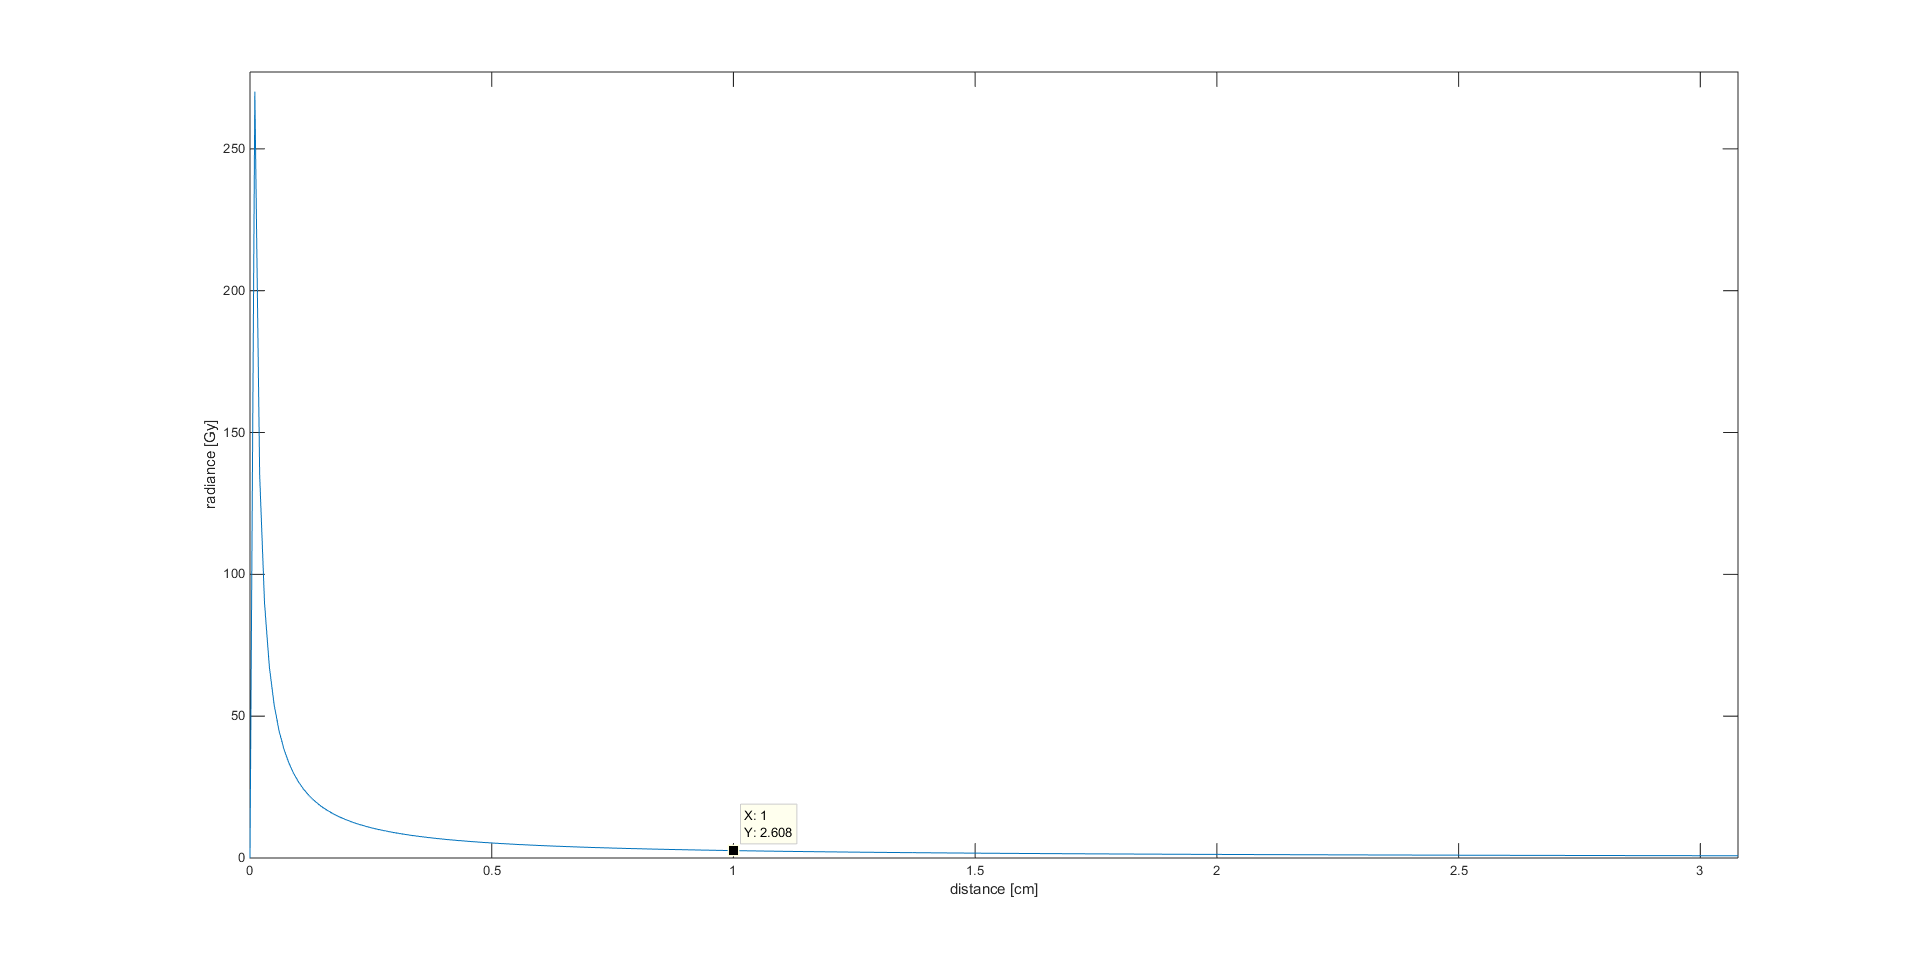
\includegraphics[width=1\textwidth]{pictures/dosefunction}
	\caption{Dose-Function Plot}
	\end{figure}
 
 
\end{frame}


\section{Algorithms}
\frame{\tableofcontents[currentsection]}
\subsection{Genetic Algorithm}
\frame{\tableofcontents[currentsubsection]}
\subsubsection{Individual}

 \begin{frame}
 \frametitle{Individual}
 The dwelltimes of the seeds are encoded in the individuals. Equation \eqref{eq:individual} shows one individual for $n  $ Seeds.
 \begin{equation}
 \label{eq:individual}
 Individual \ \ i := \begin{pmatrix}
 t_{0} \\ \vdots \\ t_{n-1} 	
\end{pmatrix}   
 \end{equation}
 \end{frame}
 
\subsubsection{Population}
 \begin{frame}
 \frametitle{Population}
 A population consists of a certain number of individuals given by the constant $ k $.
 \begin{equation}
 \label{eq:population}
 Population \ \ p := \begin{pmatrix}
 i_{0} \\ \vdots \\ i_{k-1} 	
\end{pmatrix}   
 \end{equation}
 \end{frame}
 
 \subsubsection{Fitness-Function}
 \begin{frame}
 \frametitle{Fitness-Function}
 The Fitness-Function calculates the squared differnce between the goaldose and the current dose within the whole body.
 \begin{equation}
 f(individual) = \sum_{body}(GD-CD)^2
 \end{equation}
 For further adjustment and prioritisation the Fitness-Function is extended by an weighting factor, which holds a specifig weight for any bodytype (tumor, liver, spine,...).
 \begin{equation}
 f(individual) = \sum_{body}w_{bodytype}(GD-CD)^2
 \end{equation}
 \end{frame}
 
 
 \subsubsection{Optimisation}
 \begin{frame}
 \frametitle{Optimisation}
 \IncMargin{1em}
 \begin{algorithm}[H]
 $temp=0$\;
 \For{x=0; x $\textless$ body.xDim; x++}{
 	\For{y=0; y $\textless$ body.yDim; y++}{
 		\For{z=0; z $\textless$ body.zDim; z++}{
 			\For{j=0; j $\textless$ numberOfSeeds; j++} {
				 	$temp\ \ = temp+  w_{bodytype}(GD-CD)^2$\;		
 			}
  		}
  	}
  }
 $fitnessvalue = \sqrt{temp}$\;
 \Return{fitnessvalue}\;
 \caption{Calculation of the fitnessvalue}
 \end{algorithm}
 \DecMargin{1em}
 \color{red}This causes a very high runtime...
 \end{frame}
 
 \begin{frame}
 \frametitle{Optimisation Strategies}
 Solutions to reduce the runtime:
 \begin{enumerate}
 \item Multithreading
 \item Evaluation only in a specific region around the tumor
 \item "Jump" in the for loop
 \end{enumerate}
 
 \end{frame}
 
 \begin{frame}
 \frametitle{Optimised Algorithm}
 \IncMargin{1em}
 \begin{algorithm}[H]
 \SetKwFunction{cb}{CalculateBounds}
 \SetKwFunction{thread}{ThreadedFitnessFunction}

 \emph{x-roi,y-roi,z-roi $\leftarrow$} \cb{body}  \;
 \For{x-roi}{
 	\thread{x,y-roi,z-roi}
 }
 \caption{Multithreaded Fitness-Function}
 \end{algorithm}
 \DecMargin{1em}
 
 \IncMargin{1em}
 \begin{algorithm}[H]


 \For{y=y-roi.min; y $\textless$ y-rio.max; y$\leftarrow$y+Scalefactor}{
 		\For{z=z-roi.min; z $\textless$ z-rio.max; z$\leftarrow$z+Scalefactor}{
 			\For{j=0; j $\textless$ numberOfSeeds; j++} {
				 	$temp\ \ = temp+  w_{bodytype}(GD-CD)^2$\;		
 			}
  		}
  	}
 \caption{Optimised Fitness-Function}
 \end{algorithm}
 \DecMargin{1em}
 
\end{frame}
 
\begin{frame}

\subsubsection{Elitism}
\frametitle{Elitism}
The idea of elitism is to take in every iteration the best individuals into the next iteration without any cross-over or mutation. 
\end{frame}
\subsubsection{Stop-Criterion}
\begin{frame}
\frametitle{Stop-Criterion}
The Stop-Criterion for the genetic algorithm is implemented as follows:
\IncMargin{1em}
\begin{algorithm}[H]
\SetKwFunction{iter}{GeneticAlgIteration}
$bestIndividual \leftarrow \infty $ \tcp*{FitnessValue of the best individual}  
$bestIndividualOld,currentIndividual \leftarrow 0$\;
$stop \leftarrow false$\;
$counter \leftarrow 0$\;
\While{! stop} {
 \tcc{Returns the best fitness value from the current iteration}
	$currentIndividual \leftarrow $\iter{}\;
	\If{$currentIndividual \ \   \textless \ \ bestIndividual$} {
	
		$ bestIndividual \ \   \leftarrow \ \ currentIndividual $\;
	
	}
	\If{$\left|bestIndividualOld-bestIndividual \right| \ \ \textless \ \ 1$} {
		\emph{counter++}
	} 
	\If{$counter \geq 5$} {
		$done \leftarrow true$
	}  
	
	
	
	
	}
	 

\caption{Stop-Criterion}
\end{algorithm}\DecMargin{1em}

\end{frame}

\subsubsection{Parameter}
\begin{frame}
\frametitle{Parameter Overview}
	\begin{itemize}
	\item Optimisation Paramter:
		\begin{itemize}
		\item Treatment-Range
		\item Scalefactor
		\end{itemize}
	\item Genetic Algorithm Parameter:
		\begin{itemize}
		\item Population size $k$
		\item Weighting facors $w_{bodytype}$
		\item Mutation Probability $P_{mutation}$
		\item Crossover Probability $P_{crossover}$
		\item Number of elite individuals
		\end{itemize}
	\end{itemize}
 
 
\end{frame}

\begin{frame}
\frametitle{Parameter Overview}
\textcolor{red}{parameter with influence on runtime} \\
 \textcolor{blue}{parameter with impact on optimisation quality}  
	\begin{itemize}
	\item Optimisation Paramter:
		\begin{itemize}
		\item \textcolor{red}{Treatment}\textcolor{blue}{-Range}
		\item \textcolor{red}{Scale}\textcolor{blue}{factor}
		\end{itemize}
	\item Genetic Algorithm Parameter:
		\begin{itemize}
		\item \textcolor{red}{Population} \textcolor{blue}{size $k$}
		\item \textcolor{blue}{Weighting facors $w_{bodytype}$}
		\item \textcolor{blue}{Mutation Probability $P_{mutation}$}
		\item \textcolor{blue}{Crossover Probability $P_{crossover}$}
		\item \textcolor{blue}{Number of elite individuals}
		\end{itemize}
	\end{itemize}
 
\end{frame}

\subsubsection{Runtime}
\begin{frame}
\frametitle{Runtime}
Runtime with and without optimisation\footnote{Intel\textregistered  Core i5-3570K CPU @ 4x3.40Ghz}
\begin{columns}[T] % align columns
\begin{column}{.48\textwidth}
\begin{itemize}
\item Multithreading \textcolor{red}{off}
\item $k = 10$
\item $Elitism = 2$
\item $Scalefactor = 1$
\item $Treatmentrange = 10 \ cm$
\end{itemize}

 \textbf{$\Rightarrow \ \sim $20h Runtime}
\end{column}%
\hfill%

\begin{column}{.48\textwidth}
\begin{itemize}
\item Multithreading \textcolor{green}{on}
\item $k = 10$
\item $Elitism = 2$
\item $Scalefactor = 5$
\item $Treatmentrange = 8 \ cm$
\end{itemize}

 \textbf{$\Rightarrow \ \sim $10min Runtime}
\end{column}%
\end{columns}
\end{frame}
 
 
\subsubsection{Results}
\begin{frame}
\frametitle{Results}
	\begin{figure}[h]
	\centering
	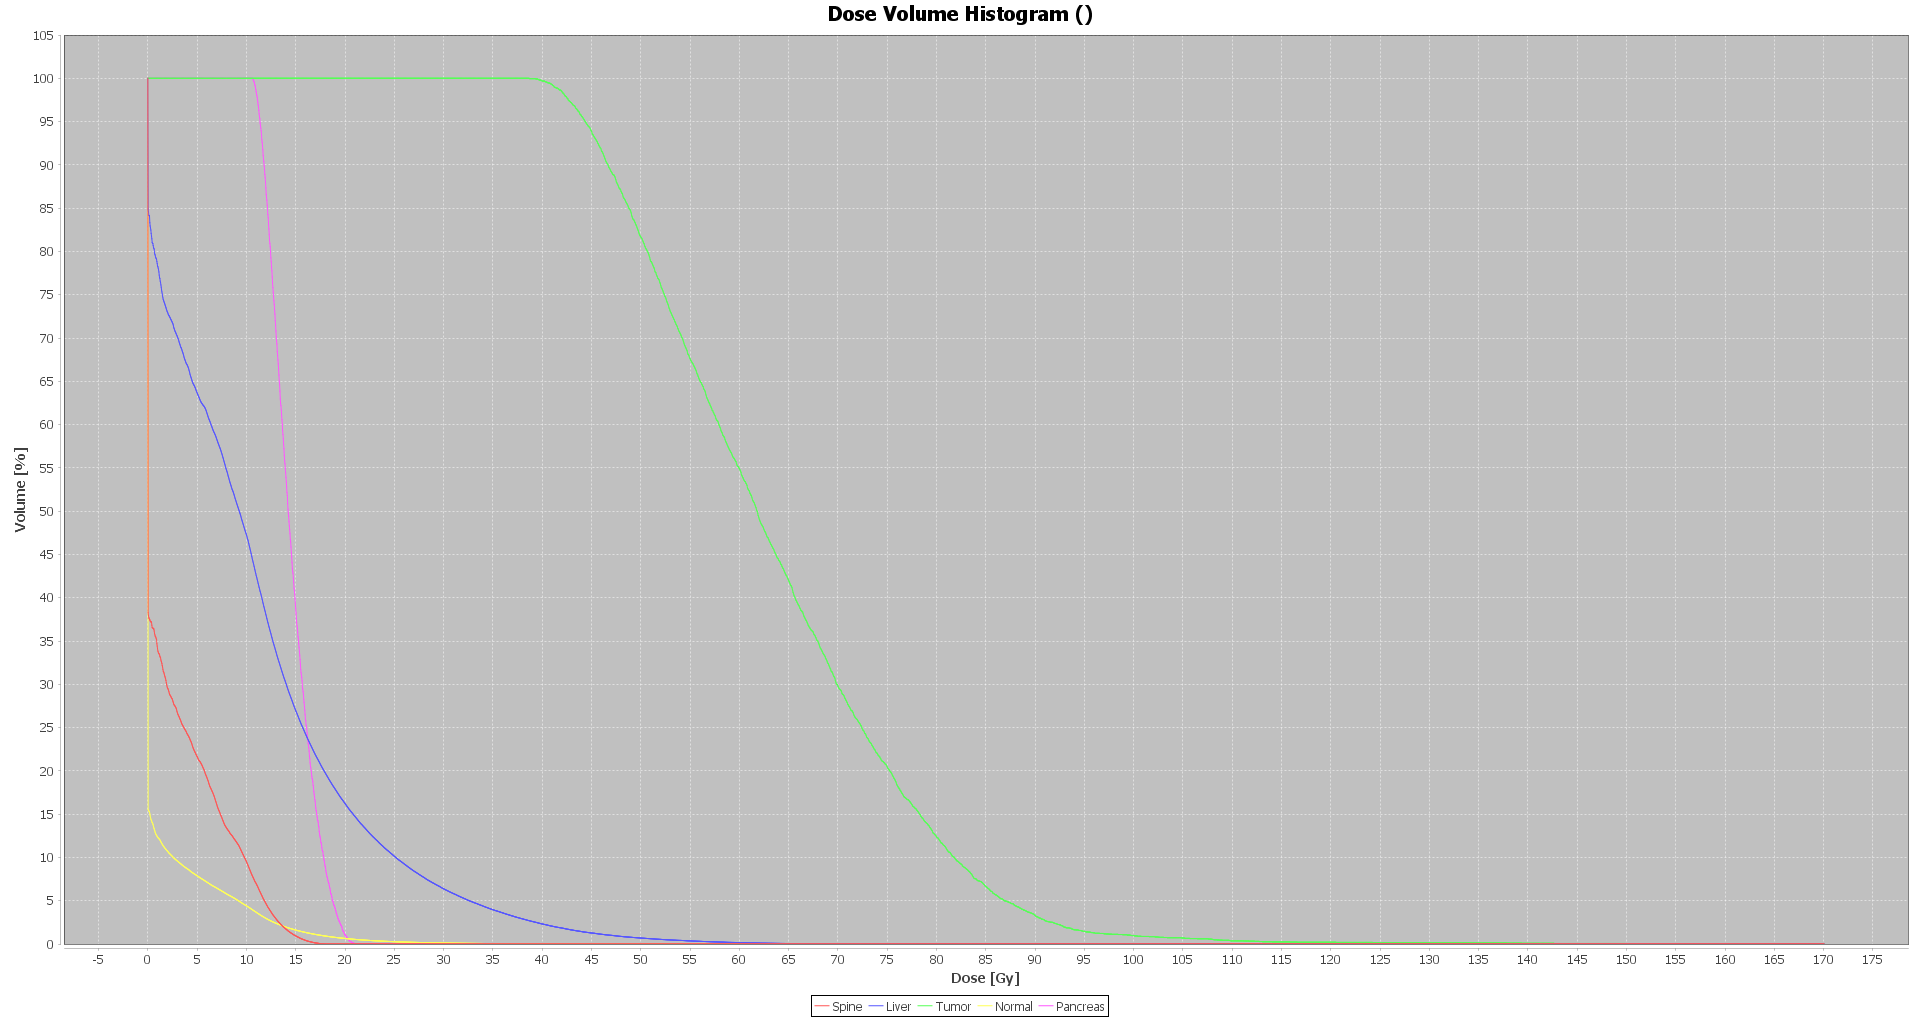
\includegraphics[width=1\textwidth]{pictures/body1_w1-4-2-3-2}
	\caption{Result of an unweighted optimisation}
	\end{figure}
 
 
\end{frame}  


\begin{frame}
\frametitle{Results}
	\begin{figure}[h]
	\centering
	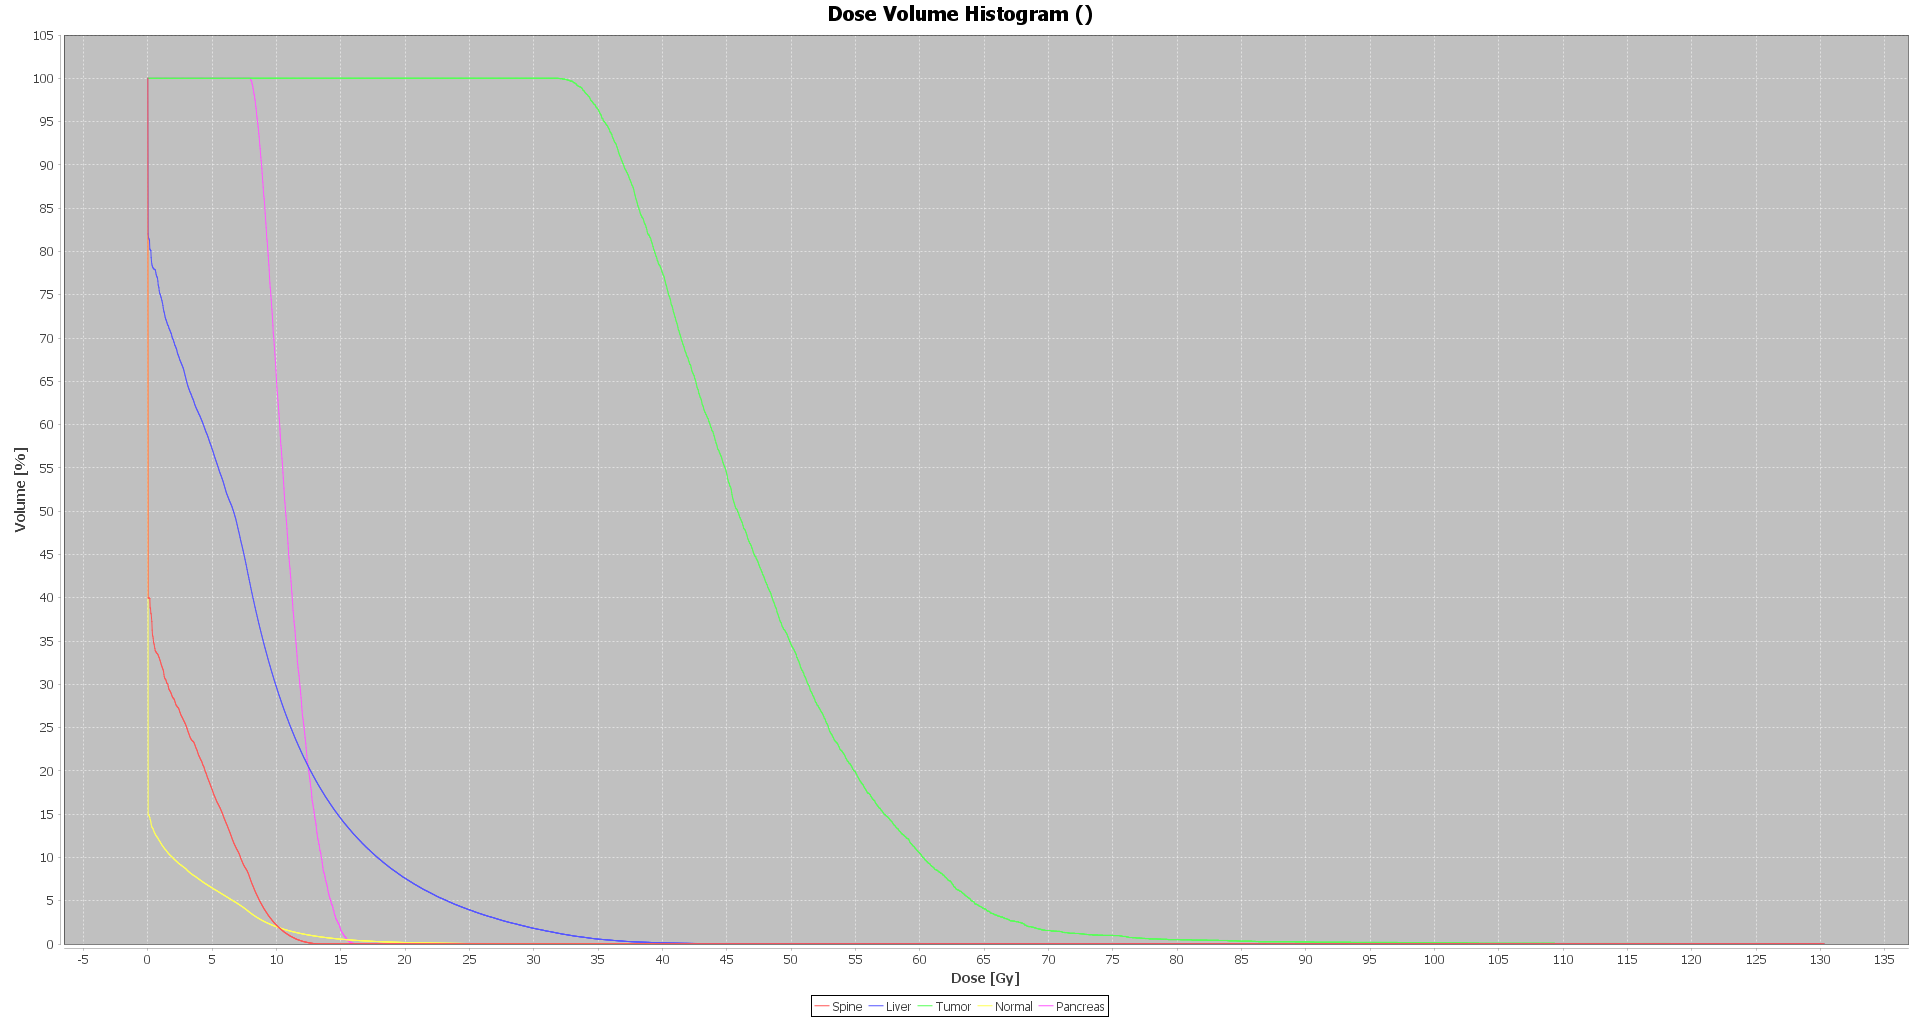
\includegraphics[width=1\textwidth]{pictures/body1_w1-4-2-70-20.png}
	\caption{Result of a weighted optimisation}
	\end{figure}
 
 
\end{frame} 


\begin{frame}
\frametitle{Results}
	\begin{figure}[h]
	\centering
	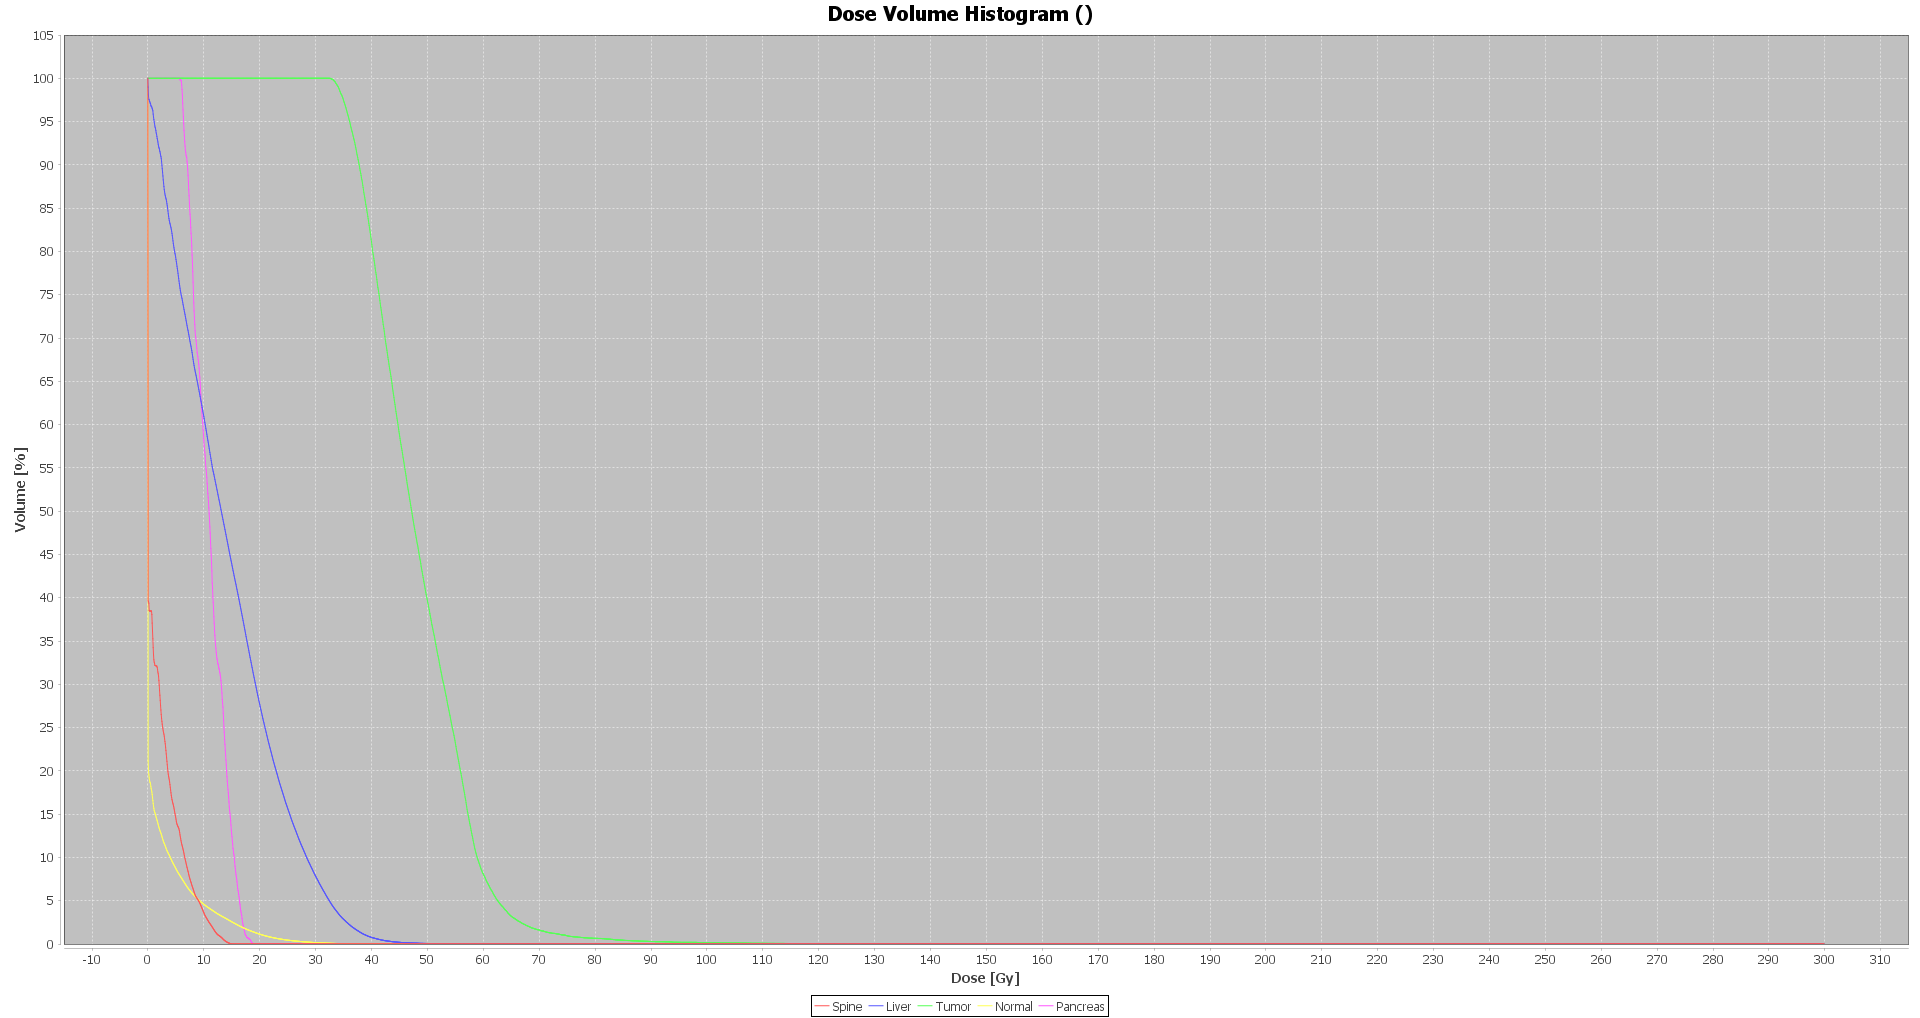
\includegraphics[width=1\textwidth]{pictures/body2_w1-4-2-70-20.png}
	\caption{Result of a weighted optimisation}
	\end{figure}
 
 
\end{frame} 

\subsubsection{Outlook}
\begin{frame}
\frametitle{Pros \& Cons}

\begin{columns}[T] % align columns
\begin{column}{.48\textwidth}
\textcolor{green}{Pros:}
\begin{itemize}
\item It always finds a good solution
\item Very flexible input
\end{itemize}

\end{column}%
\hfill%

\begin{column}{.48\textwidth}
\textcolor{red}{Cons:}

\begin{itemize}
\item Relative high runtime
\item Every patient should use individual weights for Dose-Function
\end{itemize}
\end{column}%
\end{columns}
\end{frame}

\begin{frame}
\frametitle{Outlook}
\begin{itemize}
\item Runtime/Paramter optimisation
\item Classifier for weighting factors?
\item Optimise seed positions aswell?
\end{itemize}
 
\end{frame}  
 
 
 \subsection{Linear Programming}
 \frame{\tableofcontents[currentsubsection]}
 \subsubsection{Genral Idea}
 \begin{frame}
 \frametitle{General Idea}
 \begin{figure}[h] 
  \centering
     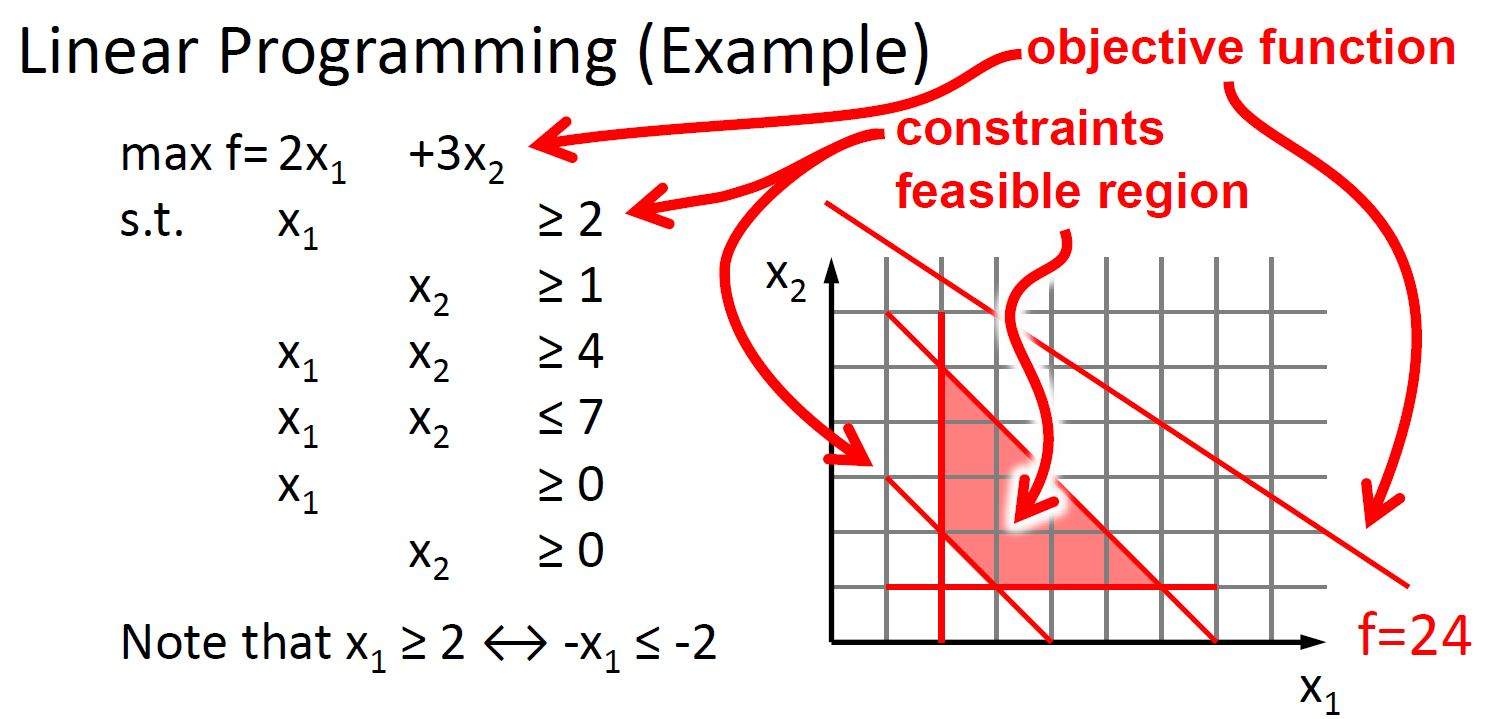
\includegraphics[width=1\textwidth]{LPexample.JPG}
  \caption{LP-Example [Intelligent Systems in Medicine - Schlaefer]}
  \label{fig:LPE}
\end{figure}
 \end{frame}
 
 \subsubsection{Objective Function - Minimize}
 \begin{frame}
 \frametitle{Objective Function - Minimize}
 The time-variable t is multiplied with the dose of the matching seed in every body fragment. The tumor is not considered.
 \begin{equation}
 \label{eq:lp}
 objective \ function: \ \ f(t_{1}, t_{2}, ... ,t_{n}) = 
 \sum_{x,y,z}^N \sum_{i=1}^n dose_{i}(body_{x,y,z}) \cdot t_{i}
 \end{equation}
 The objective function has to be minimized.
 \end{frame}
 
 \subsubsection{Constraints - Tumor}
 \begin{frame}
 \frametitle{Constraints - Tumor}
 The dose in the tumor must not fall under the defined GoalDose.
 \begin{equation}
 \label{eq:constr}
 constraints: \ \ \sum_{x,y,z}^N \sum_{i=1}^n dose_{i}(tumor_{x,y,z}) \cdot t_{i} \ge GoalDose(tumor)
 \end{equation}
 \end{frame}
 
 \subsubsection{Objective Function - Maximize}
 \begin{frame}
 \frametitle{Objective Function - Maximize}
 The time-variable t is multiplied with the dose of the matching seed in every tumor fragment. The healthy body is not considered.
 \begin{equation}
 \label{eq:lp2}
 objective \ function: \ \ f(t_{1}, t_{2}, ... ,t_{n}) = 
 \sum_{x,y,z}^N \sum_{i=1}^n dose_{i}(tumor_{x,y,z}) \cdot t_{i}
 \end{equation}
 The objective function has to be maximized.
 \end{frame}
 
 \subsubsection{Constraints - Body}
 \begin{frame}
 \frametitle{Constraints - Body}
 The dose in the healthy body must be higher then the defined GoalDose.
 \begin{equation}
 \label{eq:constr2}
 constraints: \ \ \sum_{x,y,z}^N \sum_{i=1}^n dose_{i}(body_{x,y,z}) \cdot t_{i} \le GoalDose(body_{i})
 \end{equation}
 
 Using a combination of both leads to to strong constraints. In that case the problem is not solvable.
 \end{frame}
 
 \subsubsection{Comparison}
 \begin{frame}
 \frametitle{Comparison}
 \begin{tabbing}
    only Min:....... \=blalalala \kill
    only Min: \> good tumor coverage, no modelling of body \\
    only Max: \> bad tumor coverage, good modelling of body \\
    Min-Max: \> results comparable to Max \\
    Max-Min: \> results comparable to Min, less seeds used \\
  \end{tabbing}
 \end{frame}
 
 
 \subsubsection{Using CPlex}
 \begin{frame}
 \frametitle{Using CPlex}
 
 \IncMargin{1em}
 \begin{algorithm}[H]
 $IloNumExpr \ dosepart[] \gets new \ IloNumExpr[numberOfSeeds]$\;
 $IloNumVar[] \ time \gets new \ IloNumVar[numberOfSeeds]$\;
 $IloLinearNumExpr \ objective \gets cplex.linearNumExpr()$\;

 \caption{CPlex setup}
 \end{algorithm}
 \DecMargin{1em} 
 
 \end{frame}
 
 \subsubsection*{Using CPlex}
 \begin{frame}
 \frametitle{Using CPlex}
 
 \IncMargin{1em}
 \begin{algorithm}[H]
 \For{x=0; x $\textless$ body.xDim; x++}{
 	\For{y=0; y $\textless$ body.yDim; y++}{
 		\For{z=0; z $\textless$ body.zDim; z++}{
			\If{$body[x][y][z].getBodyType() == Config.tumorType$} {
				\For{i=0; i $\textless$ numberOfSeeds; i++}{
					$dosepart[i] \gets cplex.prod(dose(x,y,z,i),time[i])$	
				}
				$cplex.addGe(cplex.sum(dosepart),goalDosis(x,y,z));$
				}
			\Else{\For{i=0; i $\textless$ numberOfSeeds; i++}{
					$objective.addTerm(dose(x,y,z,i),time[i]);$	
				}
				
				
				}
 			
  		}
  	}
  }
  $cplex.addMinimize(objective);$
  $cplex.solve();$
 \caption{CPlex}
 \end{algorithm}
 \DecMargin{1em} 
 
 \end{frame}
 
 \subsubsection*{Runtime}
 \begin{frame}
 \frametitle{Runtime}
 Runtime with different problem sizes\footnote{Intel\textregistered  Core i5-4690 CPU @ 4x3.50Ghz}
 
 
\begin{itemize}
\item $numberOfSeeds = 50 \Rightarrow \ \sim $1min Runtime
\item $numberOfSeeds = 500 \Rightarrow \ \sim $1h Runtime
\end{itemize}  
 
 The results have no significant difference.
 
 \end{frame}
 
 
\end{document}
